

\begin{abstract}[\hspace*{-10pt}]
    This chapter draws mainly on the submitted work: \fullcite{van_biesbroeck_properly_2024}  % Ce chapitre reprend principalement les travaux publiés dans: 
\end{abstract}

\begin{abstract}
    Reference priors are widely recognized for their objective nature. Yet, they often lead to intractable and improper priors, which complicates their application.
Besides, informed prior elicitation methods are penalized by the subjectivity of the choices they require. %to be made.
In this chapter, we aim at proposing a reconciliation of the aforementioned aspects. Leveraging the objective aspect of reference prior theory, we introduce two strategies of constraint incorporation to build tractable reference priors.
One provides a simple and easy-to-compute solution when the improper aspect is not questioned, and the other introduces constraints to ensure the reference prior is proper, or it provides proper posterior.
Our methodology emphasizes the central role of Jeffreys prior decay rates in this process, and the practical applicability of our results is demonstrated using an example taken from the literature.
\end{abstract}

\minitoc



\section{Introduction}\label{sec:BA:intro}


The reference prior theory represents a widely elected theory for constructing priors that are qualified as ``objective''.
The theory has been thoroughly introduced in the \cref{chap:intro-ref}. %It defines priors that maximize the impact of the observed data over themselves in the posterior definition.
The theory provides a formal mechanism to incorporate prior information in a way that maximizes the information gained from the data within the issued \emph{a posteriori} quantities.
In opposition with a plethora of existing  methods for building a prior (see e.g. \cite{mikkola_prior_2023}), 
this process is tuned to prevent the incorporation of subjective beliefs in the workflow.


However, despite their  objective nature,  their implementation is often cumbersome and not always recommended in high dimensions \citep{berger_overall_2015}. %Moreover, 
Moreover, the low-informative nature of these priors is associated with their common improper aspect, necessitating careful handling to ensure valid statistical inference.
Thus, the construction of priors is expected to strike a balance between several criteria. While many works restrict their sets of priors to ones that are tractable, proper, or suitable for high dimensions, others seek to minimize any source of subjectivity.

This chapter aims to reconcile all these criteria to improve the prior elicitation.
Our contribution takes the form of an enrichment of the reference prior theory to leverage the objective aspect that it provides to reference priors. Building on the developments presented in \cref{chap:ref-generalized},
we restrict priors to the ones that belong to  well-chosen ---and not too restrictive--- sets, and we introduce two strategies to define  convenient reference priors.
% First 
Our first strategy provides a simple,  tractable solution for constraining reference priors when the improper aspect is not questioned. The second, by contrast, introduces constraints that lead to  reference priors that are proper, or lead to proper posteriors. 
% 
For both strategies, we try to define the potential loss of objectivity induced by the constraints and we discuss their limits.
Our results emphasize the central role of Jeffreys prior decay rates when they are improper.
Additionally, we draw attention to the fact that our methodology opens a way to define various reference priors on the basis of constraints that could result from any other motivation.



This chapter is organized as follows.
In \cref{sec:BA:defsnotsmots}, after reviewing briefly the notations for the generalized reference priors framework, we develop our motivation and the objective of this work. This section is also the occasion to introduce a novel definition that is useful for the rest of the study: the quasi $D$-reference priors.
Our main results on constrained reference priors are presented in \cref{sec:BA:ress}, and discussed in \cref{sec:BA:discu}.
Then, the  practical aspect of our work is studied by the application of our method to an example taken from  the literature in \cref{sec:BA:exa}. Detailed mathematical proofs are compiled in \cref{sec:BA:proofs}. \Cref{sec:BA:conclusion} terminates the chapter with a conclusion.


\section{Definitions, notations and motivation}\label{sec:BA:defsnotsmots}

\subsection{Notations}\label{sec:BA:nots}

% \subsection{}

% notations IM, results of preceeding chapters, quasi-reference priors

%motivations %maybe its whole section

    %\subsection{The limitations of Jeffreys prior}

    %\subsection{}

In this work we consider a statistic model characterized by a collection of probability distributions $(\PP_{Y|\theta})_{\theta\in\Theta}$ on  a measurable set $(\cY,\sY)$. 
We consider the same construction of the Bayesian framework as in the \cref{chap:intro-ref} (\cref{sec:intro-refs:limits}): considering any prior $\varPi$ (that is a $\sigma$-finite measure on $\Theta$) we denote $\mbf Y_k$ a random vector of $k$ observations whose distribution conditionally to $T=\theta$ is $\PP_{\mbf Y^k|\theta}=\PP_{Y|\theta}^{\otimes k}$, where $T$ is an r.v. whose distribution is the prior $\varPi$ (see \cref{sec:intro-ref:novelframework}).

The modeling is supposed to be regular: we assume $\Theta\subset\RR^d$ with $\nu$ being the Lebesgue measure on $\RR^d$ and every prior $\varPi$ is supposed to admit a density $\pi$ w.r.t. $\nu$ (i.e. $\varPi\in\sM^\nu$).
We also assume that the model admits a likelihood, denoted by $\ell$ with for any $\theta\in\Theta$ and $\mbf y\in\cY^k$, $\ell_k(\mbf y|\theta):= \prod_{i=1}^k\ell(\mbf y|\theta)$. We suppose that it verifies \cref{assu:intro-ref:jeffreysexist} in \cref{chap:intro-ref}, making the Fisher information matrix (denoted $\cI$) and the Jeffreys prior (whose density is denoted $J$) being well-defined.
The marginal distribution (resp. density)  is denoted by $\PP_{\mbf Y_k}$ (resp. $p_{\mbf Y_k}$) and the posterior distribution (resp. density) given the observations $\mbf y\in\cY^k$ is denoted by $\PP_{T|\mbf y}$ (resp. $p(\cdot|\mbf y)$).



Given these notations, we recall the expression of the generalized mutual information, defined in the \cref{chap:ref-generalized}:
\begin{equation}
    \sI_D^k(\varPi) := \EE_{T\sim\varPi}[D(\PP_{\mbf Y_k}||\PP_{\mbf Y_k|T} )],
\end{equation}
with $D$ being a dissimilarity measure.
In this chapter, we mostly focus on such generalized mutual information when $D$ is a $\delta$ divergence with $\delta\in(0,1)$. For some $\delta\in(0,1)$, the notation $D_\delta$ will refer to the $\delta$-divergence whose expression is reminded below:
    \begin{equation}
        D_\delta(P||Q) = \int_\cX f_\delta\left( \frac{p(x)}{q(x)}  \right) q(x) d\omega(x)\quad \text{with}\quad f_\delta(x) = \frac{x^\delta-\delta x-(1-\delta)}{\delta(1-\delta)},
    \end{equation}
where $p,q$ respectively are densities pf $P$ and $Q$ w.r.t. a common measure $\omega$ on $\cX$.
When evoking reference priors in a general way, we will refer to generalized reference priors, as proposed in the \cref{chap:ref-generalized}.
We remind below their definition:
\begin{defi}[Generalized reference prior]\label{def:BA:genref}
    Let $D$ be a dissimilarity measure and $\cP$ a set of priors on $\Theta$. A prior $\varPi\in\cP$ is called a $D$-reference prior over $\cP$ with rate $\varphi(k)$ if there exists an openly increasing  sequence of compact subsets $(\Theta_i)_{i\in\NN}$
    such that $\bigcup_{i\in\NN}\Theta_i=\Theta$ and for any $i$: $0<\varPi(\Theta_i)<\infty $ and
    % with $\pi^\ast(\Theta_i)>0$, $\Theta_i\subset\Theta$, $\bigcup_{i\in I}\Theta_i=\Theta$ such that
        \begin{equation} %\label{eq:defrefpriorsi}
            \lim_{k\rightarrow\infty}\varphi(k)[\sI^k_D(\varPi(\cdot|\Theta_i))-\sI^k_D(P(\cdot|\Theta_i))] \geq0 \text{\ for all\ } P\in\cP\text{\ verifying\ }0<P(\Theta_i)<\infty;
        \end{equation}
    where  $\varphi(k)$ is a {positive and}  monotonous function of $k$. It is said to be unique if for any other $D$-refernce prior $\varPi'$, $\varPi\simeq\varPi'$.
\end{defi}

We also remind the following result on the $D_\delta$-mutual information and their reference priors (see \cref{chap:ref-generalized}).
%  that are defined considering a generalized ,
\begin{thm}\label{thm:BA:l(pi)}
    Suppose $\Theta$ to be compact and $\varPi\in\sM^\nu_\cC$ be a prior with $\varPi(\Theta)=1$. the $D_\delta$-mutual information admits a limit:
        \begin{equation}
            \lim_{k\rightarrow\infty} k^{d\delta/2} \sI_{D_\delta}(\varPi) = l(\pi) - (\delta(1-\delta))^{-1}, \quad l(\pi) = C_\delta \int_{\Theta}\pi(\theta)^{1+\delta} |\cI(\theta)|^{-\delta/2}  d\theta ,
        \end{equation}
        where $\pi$ is the density of $\varPi$, and with $C_\delta= (2\pi)^{d\delta/2} (1-\delta)^{-d/2}/(\delta(\delta-1))$.\\
    Call $\cR\subset\sR_{\cC^b}$ a set of densities such that $M(\cR)=\cP$, with $M$ mapping a density to its associated prior. Then
        $\varPi$ is a $D_\delta$-reference prior over $\cP$ iff $\pi$ maximizes $l$ over $\cR$. 
\end{thm}




\subsection{Objective and motivation}\label{sec:BA:mots}



We already know that the definition of the reference prior and the $D_\delta$-reference prior is satisfied by the Jeffreys prior over the large set of priors $\sM^\nu_\cC$ in most cases (see \cref{chap:intro-ref,chap:ref-generalized}).
% in most case (see \cref{chap:intro-ref} for ). 

%the large set of priors admitting locally bounded and a.e. continuous densities w.r.t. the Lebesgue measure \citep{VanBiesbroeckBA2023}. 

This result is, however, limiting and disappointing in some cases. The reasons are the following ones: (i) the Jeffreys prior is not recommended in high-dimensional problems as it is known to be ``either too diffuse or too concentrated'' \citep{berger_overall_2015}; moreover (ii) when the expression of the likelihood is itself complex, the computation of the Jeffreys prior can become  intractable; %which is why (iii) in practice a restriction to the set of priors to ones which are easier to compute is often favored; 
also (iii) the Jeffreys prior is known to often lead to an improper prior, which does not necessarily issue a proper posterior distribution, essential for practical \emph{a posteriori} inference and sampling.

To tackle these limitations, we propose in this work to restrict the set of priors over which we derive the reference priors.
Indeed, the reference prior definition is usually considered with very large sets of priors, which are constrained only by some regularity assumptions imposed to the priors (such as continuity, positivity). These regularity assumptions do not generally discriminate the Jeffreys prior from the studied set of priors.
In this chapter, different restricted sets of priors will be suggested, they are sets that are though 
to counter the limitations (ii) and (iii) aforementioned. In most cases, they will not include the Jeffreys prior.
%to not include the Jeffreys prior when 



The tackling of limitation (i) mentioned above is not a purpose of this work. We recall that it is actually frequently tackled by a sequential construction of the reference prior as %presented in \cref{chap:intro-ref} (\cref{sec:intro-ref:refpriors}).
suggested by \citet{bernardo_reference_1979}.
On the condition that an ordering of the parameters is set:
 \begin{equation}
     \theta = (\theta_1,\dots,\theta_r) \in \Theta=\Theta_1\times\dots\times\Theta_r,
 \end{equation}
this construction considers a hierarchical construction of the reference prior.
It is already described in \cref{chap:intro-ref} (\cref{sec:intro-ref:refpriors}). We remind below the steps of the sequential construction:
%
%Typically, it is recommended to assume $\Theta_j\subset\RR^{d_j}$ with small dimensions $d_j$ (e.g., lower or equal than $2$) for any $j\in\{1,\dots,r\}$, and to sequentially build a reference prior on the $\Theta_j$,  $j\in\{1,\dots,r\}$:
 \begin{enumerate}
     \item initially fix $\ell_k^1=\ell_k$;
     \item for any values of $\theta_{j+1},\dots,\theta_r\in\Theta_{j+1}\times\dots\times\Theta_r$, compute a reference prior (in the sense of \cref{def:intro-ref:ref-priors})  under the model with likelihood $\theta_j\mapsto\ell_k^j(\mbf y|\theta_j,\dots,\theta_r)$, denote $\pi_j(\cdot|\theta_{j+1},\dots,\theta_r)$ its normalized density;
     \item derive $\ell_k^{j+1}$ such as 
         \begin{equation} %\label{eq:hier:condlikeint}
            \ell_k^{j+1}(\mbf y|\theta_{j+1},\dots,\theta_r) =  \int_{\Theta_j}\ell_k^j(\mbf y|\theta_j,\dots,\theta_r)d\pi_j(\theta_j|\theta_{j+1},\dots,\theta_r).
         \end{equation}
 \end{enumerate}

In this work, the reference priors will be derived only given their formal definition (\cref{def:BA:genref}). Yet, our results can be incorporated in this sequential construction. Indeed,
step 2 of the method depicted above consists of the derivation of a reference prior w.r.t. the variable $\theta_j$.
%in the sense of 
% Thus, our reference priors over constrained setes of priors can be  plainly incorporated into this method.
Additionally, we invite to note that this construction does not solve the limitations (ii) and (iii) previously evoked. Actually, it makes them essential. Indeed, step 2 requires, firstly, a derivation of a reference prior, so that it would lead to a low-dimensional Jeffreys prior if the set of priors is not constrained. Also step 3 necessitates, secondly, that the latter leads to a proper posterior so that the integral involved does not diverge.

We note that this last issue is taken into account by \citet{berger_development_1992} with the suggestion of such construction on an increasing sequence of compact subsets of $\Theta$: $\bigcup_{i\in\NN}\Theta_i=\Theta$. The hierarchical reference prior can then be chosen as a limit of the ones obtained under $\Theta_i$ when $i\to\infty$. However, this limit can be cumbersome to derive in practice. Another solution suggested by \citet{mure_objective_2018} is to restrict the $\sigma$-algebra $\sY$ until the reference prior derived in step 2 leads to a proper posterior. It is still imperfect, as there is no guarantee that such a restricted $\sigma$-algebra exists outside the trivial one.


%In the following subsections, we propose a range of solutions to some of the issues aforementioned, based on the derivation of reference priors over constrained setes of priors. In  Section  {sec:constrainedasympt}, we derive a quasi $D_\delta$-reference prior over setes of priors that are easy to compute, in order to tackle the limitations (ii) and (iii) previously evoked. Then, Section  {sec:constrainedproper} explores another kind of constrained setes of priors, which leads to $D_\delta$-reference priors that can solve the item (iv).












\subsection{A useful definition: quasi-reference priors}\label{sec:BA:defsquas}

%As explained in the introduction, the objective of this work is to study reference priors over restricted sets of priors. Indeed, the reference prior definition is usually considered with very large sets of priors, which are constrained only by some regularity assumptions imposed to the priors (such as continuity, positivity). %This regularity does not generally discriminate the Jeffreys prior
%Actually, 
%The choice of the set of priors $\cP$ in \cref{def:BA:genref} remains open and can be restrained from the large one of priors in $\cM^\varrho_\cC/\!\simeq$. %admitting continuous densities w.r.t. the Lebesgue measure.

While we aim at restricting the set of priors $\cP$ in \cref{def:BA:genref}, we must notice
that such a restriction leaves really unsure the existence of a reference prior. 
Indeed, the definition is itself restrictive, as to admit a reference prior, the set $\cP$ must contain a prior whose restrictions are optimal on any compact subsets of $\Theta$.
In this section, we suggest an extension of the definition of reference priors in the case where in the set $\cP$, the optimal priors on compact subsets of $\Theta$ are not renormalization of each other, but converge to a  prior in $\cP$. 
Such convergence is considered in the sense of the Q-vague convergence \citep{bioche_approximation_2016} on $\sM^\nu_\cC$. % on $\cM^\nu\cC/\!\simeq$. This convergence defines a topology 
The Q-vague convergence of a sequence $(\varPi_n)_n$ to a limit $\varPi$ is equivalent to the convergence of $([\varPi_n])_n$ to $[\varPi]$ in $\sM^\nu_\cC/\!\simeq$ for the quotient topology of the vague convergence on $\sM^\nu_\cC$.




\begin{defi}[Quasi reference prior]\label{defi:quasiRefprior}
    Let $\cP$ be a set of priors. We call $\varPi\in\cP$ a quasi $D$-reference prior if it exists an openly increasing sequence $(\Theta_i)_{i\in \NN}$  of compact sets with $\bigcup_{i\in\NN}\Theta_i=\Theta$ such that
    \begin{itemize}
        \item[(i)] for any $i\in \NN$, there exists a $D$-reference prior $\varPi_i$ over $\cP_i=\{P(\cdot|\Theta_i),\, P\in\cP,\,P(\Theta_i)\in(0,\infty) \}$, %, the set of renormalized restrictions to $\Theta_i$ of priors in $\cP$,
        \item[(ii)] $\varPi$ is the Q-vague limit of the sequence $(\varPi_i)_{i\in \NN}$.
    \end{itemize}
    It is said to be unique  if for any other quasi $D$-reference prior $\varPi'$, $\varPi\simeq\varPi'$.
\end{defi}

Proposition below ensures that this definition properly extends \cref{def:BA:genref} in the case of $\delta$-divergences.
\begin{prop}\label{prop:quasi}
     \begin{itemize}
        \item If $\varPi$ is a $D_\delta$-reference prior over a set $\cP$, then it is a quasi $D_\delta$-reference prior.
        \item If $\cP$ is a set of priors convex and stable by multiplication by indicator functions over measurable sets, then the quasi $D_\delta$-reference prior over $\cP$ is the unique $D_\delta$-reference prior over $\cP$.
        \item If $\cP$ is a convex set of priors and if the sequence of subsets $(\Theta_i)_i$ in \cref{def:BA:genref} is fixed, then the quasi-reference prior over $\cP$ is unique.
    \end{itemize}
\end{prop}


\begin{proof}
    The first statement of the proposition is clear given the definition of a $D_\delta$-reference prior.\\
    For the second, let us adopt the notations of \cref{thm:BA:l(pi)} and  notice that if $\Theta$ is compact and if $\pi^\ast$ is the maximal argument of $l$ over $\cR$, then its renormalized restriction $\pi_1^\ast$ on a compact subset $U$ maximizes $l$ over the set of all renormalized densities $\cR_U$.
    Indeed, if we suppose that $\pi_1\in\cR_U$ maximizes $l$ then, denoting $\pi_0^\ast$ the renormalized restriction of $\pi^\ast$ to $\Theta\setminus U$, $t=\int_U\pi^\ast$, and $\pi = t\pi_1+(1-t)\pi_0^\ast$, $\pi\in\cR$ and
        \begin{equation}
            l(\pi) = t^{\delta+1}l(\pi_1) + (1-t)^{\delta+1}l(\pi_0^\ast) > t^{\delta+1}l(\pi_1^\ast) + (1-t)^{\delta+1}l(\pi_0^\ast) = l(\pi^\ast).
        \end{equation}
    Hence $\pi^\ast$ does not maximize $l$ over $\cR$, which is absurd.\\
    Therefore, in our problem, considering two sequences $(\pi^{(1)}_i)_i$ and $(\pi_i^{(2)})_i$ respectively defined on $(\Theta_i^{(1)})_i$ and $(\Theta^{(2)}_i)_i$, we will get that for any $i$, $\pi^{(1)}_i(\theta)=\pi_i^{(2)}(\theta)$ for all $\theta\in\Theta_i^{(1)}\cap\Theta_i^{(2)}$. Eventually, they are identical on every compact subsets of $\Theta$, and equal to their Q-vague limits which are the same.\\
    Finally, the third statement of the proposition results from the strict concavity of $l$. Indeed, for any $i$, the set $\cR_i$ of renormalized restricted densities on $\Theta_i$ is convex so that the maximal argument of $l$ over $\cR_i$ is unique. Hence the uniqueness of the quasi-reference prior over $\cP$.
\end{proof}
    



\section{Constrained $D_\delta$-reference priors}\label{sec:BA:ress}


In this section, we present results of two different constraint incorporation on the reference priors.
In \cref{sec:BA:res1}, the constraint limits the set of priors to exponentiation of coordinates of $\theta$. The result suggests a simpler reference priors in a case where the improper Jeffreys prior's decay rates are not an issue.
%When the Jeffreys prior has an improper asymptotic behavior that matches with a prior in this set, we show that
In \cref{sec:BA:res2}, we introduce a well-chosen linear constraint on the set of priors that ensures the constraint reference prior is proper, or leads to proper posteriors.

%Our first strategy provides a simple,  tractable solution for constraining reference priors when the improper aspect is not questioned. The second, by contrast, introduces constraints that lead to  reference priors that are proper, or lead to proper posteriors. 


\subsection{Constrained $D_\delta$-reference priors based on Jeffreys' asymptotic decay rates}\label{sec:BA:res1}



    % \subsection{Results}

    


    In this section, we tackle the computational cost of the reference prior. As mentioned in \cref{sec:BA:mots}, the Jeffreys prior expression is often complex to derive even in low dimensional models. This is even more a problem in practical studies where the prior must be evaluated a numerous number of times, when it resorts to MCMC simulations to provide posterior samples of $\theta$ for instance.

    In some works of the literature, the Jeffreys prior is replaced by its decay rates at the boundary of the domain. For instance, the reference prior for Gaussian processes suggested by \citet{gu_jointly_2019} is built on the basis of the decay rates of a Jeffreys prior sequentially computed on the different variables that compose $\theta$ (following the construction presented in \cref{sec:BA:mots}).
    Their idea is that, in particular when it is improper, the prior provides the most information from its asymptotic rates, and variations of them are noticed to have a strong influence on the posterior distribution.
    The result that follows provides a formalization of this intuition, focusing on the case where the Jeffreys prior asymptotically behaves like exponentiation of coordinates of $\theta$.
    
    
    
    
    
    \begin{thm}\label{thm:Jthetaa}
        Suppose $\Theta\subset\RR$ is an interval of the form $[c,b)$ (or $(b,c]$). Call $M:\pi\in\sR_{\cC^b}\mapsto(B\mapsto\int_B \pi d\nu)\in\sM^\nu_\cC$. %, with $J$ integrable and non-null in the neighborhood of $c$.
        \begin{itemize}
            \item If $b\in\RR$ and $J(\theta)\equi{\theta\rightarrow b}C|\theta-b|^a$ for constants $C\in\RR$ and $a\leq-1$, then $M(\pi^\ast)$ where $\pi^\ast(\theta)\propto|\theta-b|^a$ is the unique quasi $D_\delta$-reference prior over $M(\hat\cR)$ where $\hat\cR = \{\pi(\theta)\propto|\theta-b|^u,\,u\in\RR\}$.
            \item If $|b|=\infty$ and $J(\theta)\equi{\theta\rightarrow b}C\theta^a$ for constants $C\in\RR$ and $a\geq-1$, then $M(\pi^\ast)$ where $\pi^\ast(\theta)\propto\theta^a$ is the unique quasi $D_\delta$-reference prior over $M(\hat\cR)$ where $\hat\cR = \{\pi(\theta)\propto\theta^u,\,u\in\RR\}$.
        \end{itemize}
    \end{thm}
    
    \begin{proof}
        The proof is technical and detailed in \cref{sec:BA:proofs}.
        The idea is that $l(\pi)$ can be seen as a negative divergence between $\pi$ and $J$. However, when $J$ is improper at the boundary of the domain, the maximization of $l(\pi)$ gets closer to the minimization of a divergence between $\pi$ and the improper decay rate of $J$.
    \end{proof}
    
    
    \begin{rem}
        \Cref{thm:Jthetaa} still stands when $\Theta=(b,c)$ (or $(c,b)$) if $c\ne\infty$ and if $J(\theta)$ admits a non-null and finite limit when $\theta\to b$.
    \end{rem}
    
    
    
    
    This theorem serves the statement of two conclusions: (i) it emphasizes that when Jeffreys prior is improper, its improper decay rates contain the most relevant information, and (ii) it proposes to choose this asymptotic expansion of Jeffreys as a quasi $D_\delta$-reference prior when we look for an easy prior to compute.
    
    
    






\subsection{Properly constrained $D_\delta$-reference priors}\label{sec:BA:res2}



In \cref{sec:BA:res1}, we have provided some elements to construct a tractable reference prior on the coordinates over which Jeffreys prior is improper.
The reference prior that our theorem proposes keeps the improper characteristic of Jeffreys prior on the same coordinates.
This improper aspect can, however, remain an issue in some cases, especially when the resulting posterior is improper as well.

For this reason, it might happen that some asymptotic rates in some directions still have to be tackled. The work in this section is concluded by results that allow defining a $D_\delta$-reference prior (or quasi $D_\delta$-reference prior), which benefits from adjusted decay rates from Jeffreys prior. 
The proposition below constitutes a preliminary result that gives the form of a $D_\delta$-reference prior over a set of priors with linear constraints.

\begin{assu}\label{assu:glibre}
    A family of functions from $\Theta$ to $\RR$ $(g_j)_{j=1}^p$ is said to satisfy \cref{assu:glibre} if $g_0,\dots,g_p$ are linearly independent in the space of a.e. continuous functions from $\Theta$ to $\RR$, where $g_0:=\theta\mapsto 1$.
\end{assu}

\begin{prop}\label{prop:constraints}
    Suppose $\Theta$ to be a compact subset of $\RR^d$. Let $g_1,\dots,g_p$ be %a.e. continuous 
    functions in $\sR_{\cC^b}$ %from $\Theta$ to $\RR$ 
    that satisfy \cref{assu:glibre}. Define $\tilde\cP$ the set of priors $\varPi$ on $\Theta$ such that $\forall 1,\dots,p$, $\int_\Theta g_jd\varPi=c_j$, for some $c_j\in\RR$.
    If %$\tilde\cP$ is not empty, then 
    there exists a $D_\delta$-reference prior over $\tilde\cP$, it is unique. If it is positive, its density $\pi$ verifies
    \begin{equation}
        \pi(\theta) = J(\theta)\left(\lambda_0+\sum_{j=1}^p\lambda_jg_j(\theta) \right)^{1/\delta},
    \end{equation}
    for some $\lambda_j\in\RR$. Reciprocally, if there exists a prior %$\pi^\ast\in\tilde\cP$ 
    whose density verifies the above equation for some $\lambda_j\in\RR$, it is the $D_\delta$-reference prior over $\tilde\cP$.
\end{prop}

\begin{proof}
    This proposition results from a Lagrange multipliers theorem. A detailed proof is proposed in \cref{sec:BA:proofs}.
\end{proof}



\begin{rem}
    While it is not the subject of this work, we let the reader notice that this proposition opens the way to the introduction of constraints based on expert judgments in prior elicitation. They can take the form of moment constraints or predictive constraints. %\citep{bousquet_contributions_2024}.    
\end{rem}

\begin{rem}\label{rem:klconst}
    The expression of the reference prior given by \cref{prop:constraints} depends on the chosen $\delta$-divergence.
    While this work considers only the framework of reference priors under $\delta$-divergences as a dissimilarity measure, a version of this theorem could be written in the original framework of the reference prior theory that uses the Kullback-Leibler divergence. The expression of the resulting reference prior would be impacted. 
    In the appendix we prove that the expression using the Kullback-Leibler divergence would take the form:
    %In \cite{bernardo_bayesian_1994}, the authors suggest that the expression should take the form of
        \begin{equation}
            \pi^\ast\propto J\cdot\exp\left(\sum_{j=1}^p\lambda_j g_j\right),
        \end{equation}
        for some $\lambda_j$ that remain to be determined.
    This expression was already intuited by \citet{bernardo_bayesian_1994}.
        %Their suggestion is supported by the derivations made in \cite[\S C.3, Theorem 2]{GauchyPhD}.
\end{rem}
 



Below, given a function $g$ that is selected to adjust the asymptotics of Jeffreys prior, is stated the expression of a proper $D_\delta$-reference prior.

\begin{thm}\label{thm:lintoproper}
    Let $g:\Theta\to(0,\infty)$ be a function in $\sR_{\cC^b}$ such that
        \begin{equation}\label{eq:intgalphafinite}
            \int_\Theta J(\theta)g^{1/\delta}(\theta)d\theta<\infty \quad\text{and}
            \quad\int_\Theta J(\theta)g^{1/\delta+1}(\theta)d\theta<\infty,
        \end{equation}
    and suppose that $g$ is bounded in the neighborhood of $b$ for an element $b\in\partial\Theta$. %such that $J$ is improper in the neighborhood of $b$.
    We denote by $\overline\cP$ the set of positive priors $\varPi$ on $\Theta$ such that $\int_\Theta gd\varPi<\infty$, and we define 
    $\varPi\in\overline\cP$ as the prior whose density $\pi$ verifies % follows 
        \begin{equation}
            \pi(\theta)\propto J(\theta)g(\theta)^{1/\delta}.
        \end{equation}
    If $Jg$ is non-integrable in the neighborhood of $b$, then $\varPi$ is a $D_\delta$-reference prior over $\overline\cP$. Otherwise, and if $J$ is improper in the neighborhood of $b$, $\varPi$ is a $D_\delta$-reference prior over the set of proper priors in $\overline\cP$.
\end{thm}

\begin{proof}
    The statement of this theorem results from the sequential use of \cref{prop:constraints} on an increasing sequence of compact subsets of $\Theta$. A detailed proof is written in \cref{sec:BA:proofs}.     
\end{proof}


%\begin{rem}
   To improve the above theorem, one would like 
     to relax the first assumption in \cref{eq:intgalphafinite}, i.e., to let $\int_\Theta J g^{1/\delta}$  be infinite. Indeed, in this way, the result would provide a reference prior $\varPi$ ---non-necessarily proper--- but such that $\pi g\in L^1$, where $\pi$ is a density of $\varPi$. With a good choice of $g$, $\pi^\ast$ could be built as a prior that provides a proper posterior. It is the purpose of the next theorem. 
    The cost of this relaxation is the provision of a quasi-reference prior instead of a reference prior.
    %However, our proof needs this assumption, but one can feel that such (quasi)-reference prior is not far to exist as expressed in the proposition  below.
%\end{rem}

\begin{thm}\label{thm:quasipostpropre}
    Let $g:\Theta\to(0,\infty)$ be in $\sR_{\cC^b}$ such that
    \begin{equation}
        \int_\Theta J(\theta)g(\theta)d\theta=\infty\quad\text{and}\quad \int_\Theta J(\theta)g^{1/\delta+1}(\theta)d\theta<\infty,
    \end{equation}
and suppose that $g(\theta)\conv{\theta\rightarrow b}0$ for an element $b\in\partial\Theta$ such that $J$ is non-integrable in the neighborhood of $b$.\\
Let $(\Theta_i)_{i\in\NN}$ be an openly increasing sequence of compact sets that covers $\Theta$ and $(c_i)_i$ be a bounded sequence in $(0,\infty)$. Define the set of priors  $\overline\cP'=\{\varPi,\,\forall i,\,\int_{\Theta_i} gd\varPi=c_i\int_{\Theta_i}d\varPi\}$.\\ %, where $(c_i)_i$ is a bounded sequence in $(0,\infty)$.\\
Denote for any $i$ $\overline{\cP}'_i$ the set of renormalized restrictions to $\Theta_i$ of priors in $\overline{\cP}'$. If for any $i$ there exists a  positive maximum of $l$ over $\overline\cP'_i$, then  $\varPi$ whose density is denoted $\pi$ is a quasi $D_\delta$-reference prior over $\overline\cP'$ with
    \begin{equation}
        \pi(\theta)\propto J(\theta)g(\theta)^{1/\delta}.
    \end{equation}
    This prior is such that $\int_\Theta\pi gd\nu<\infty$.
\end{thm}




\section{Discussion}\label{sec:BA:discu}

The knowledge of Jeffreys prior's decay rates is central in the results presented in this work. These results indicate that in common scenarios where Jeffreys prior is improper, these rates must be explicitly considered in order to construct a reference prior. 

We let the reader note that \cref{thm:lintoproper,thm:quasipostpropre} introduce results that also depend on the chosen dissimilarity measure. Therefore, a balance must be found between the subjective influence of the constraint and the quest for an informed prior to facilitate possible sampling from the posterior. This is illustrated in the example we address in the following section.
However, it is important to observe that using the KL-divergence instead of a $\delta$-divergence %considered in our work 
would result in a stronger influence of the constraint on the final prior. As noted in \cref{rem:klconst}, the exponentialization of the function $g$ could lead to a prior with distribution tails that are significantly negligible beyond those of Jeffreys, thereby jeopardizing its objective nature.

Generally, the results we propose in \cref{sec:BA:res1,sec:BA:res2} address different problems and are thus  fundamentally different in nature. In one case, the improper aspect of Jeffreys prior is not necessarily challenged, and an efficient construction of the latter is proposed. In the other case, the goal is to significantly attenuate its improper aspect while maintaining as much objectivity as possible. In this latter case, however, the expressions of the proposed  reference priors still depend on the expression of Jeffreys prior. Nevertheless, when Jeffreys prior is proper, there is no guarantee that a straightforward construction inspired by its convergence rates at the domain boundaries will be relevant. %ensure its reference nature in a simple and interpretable way. 
Indeed, although improper tails concentrate an infinite mass that constitutes all the information at the boundaries, when they are proper, the information of interest may need to be sought elsewhere. In this case, a calculation or approximation of the `proper' Jeffreys prior remains to be considered.

Finally, regarding \cref{thm:Jthetaa}, although the result is limited to parameter power distribution tails, it is observed that, in practice, these include a wide range of improper Jeffreys priors.
For example, this includes Jeffreys priors derived from various Gaussian models, such as those introduced by \citet{neyman_consistent_1948}; Jeffreys priors related to specific parameters within Gaussian process models \citep{gu_parallel_2016}; and those arising in more specialized contexts, like the one %
that we develop in the \cref{part:spra} of this manuscript.
%in \cite{VanBiesbroeck2023}.
%
%
%are concerned the Jeffreys prior in the normal 
%\textcolor{red}{Il faudrait en lister plusieurs.}
Moreover, the invariance of Jeffreys priors under re-parameterization can sometimes allow us to return to this case. Specifically, if $J$ can be asymptotically written as a power of a function $f$, where $f$ is differentiable, monotone and with bounded derivative (from above and from below), then the re-parameterization $\vartheta=f(\theta)$ %with a well  
should allow us to recover the reference prior among those expressible as powers of $f$.

In the following section, we illustrate an application of our work with an example taken from the literature.


\section{An example}\label{sec:BA:exa}


In their work, \citet{rubio_inference_2014} prove that the two piece location-scale model they proposed has an improper Jeffreys prior, which issues an improper posterior.
The model is parameterized by $\theta=(\mu,\sigma_1,\sigma_2)\in\RR\times(0,\infty)^2$, inferred over observations in $\cY=\RR$. It has the following likelihood:
    \begin{equation}\label{eq:examplelikilihood}
        \ell(y|\theta) =  \frac{2}{\sigma_1+\sigma_2}\left[f\left(\frac{y-\mu}{\sigma_1}\right)\indic_{(-\infty,\mu)}(y) + f\left(\frac{y-\mu}{\sigma_2}\right)\indic_{(\mu,\infty)}(y)  \right],
    \end{equation}
where $f$ is a density function with support on $\RR$, assumed to be symmetric with a single mode at zero, and with a few integrability assumptions that are detailed in \cite{rubio_inference_2014}.
    The choice of $f$ is open and we can take, % let the assumptions of Theorem  {thm:l(pi)} to be verified.
    %\textcolor{red}{
    %We may take, 
    for instance, the standard Gaussian density function.
    Under this construction, the Fisher information matrix of this model takes the form:
    \begin{equation}\label{eq:fishermatrix}
        \cI(\theta) = \left(\begin{array}{ccc}
             \frac{\alpha_1}{\sigma_1\sigma_2}& -\frac{2\alpha_3}{\sigma_1(\sigma_1+\sigma_2)} & \frac{2\alpha_3}{\sigma_2(\sigma_1+\sigma_2)}  \\
             \ast &\frac{\alpha_2}{\sigma_1(\sigma_1+\sigma_2)} + \frac{\sigma_2}{\sigma_1(\sigma_1+\sigma_2)^2} & - \frac{1}{(\sigma_1+\sigma_2)^2}  \\
             \ast&\ast& \frac{\alpha_2}{\sigma_2(\sigma_1+\sigma_2)} + \frac{\sigma_1}{\sigma_2(\sigma_1+\sigma_2)^2}
        \end{array}\right)
    \end{equation}
    for some positive constants $\alpha_1$, $\alpha_2$ and $\alpha_3$.

    The full Jeffreys prior can be computed as 
    \begin{equation}
        J(\theta) \propto \frac{1}{\sigma_1\sigma_2(\sigma_1+\sigma_2)},
    \end{equation}
    it is improper and leads to an improper posterior. In the following, we construct different priors based on the suggestions developed in this chapter. %a method which, on the basis of our suggestions developed in what precedes, to construct a more suitable prior.

    \paragraph{Proper priors based on a moment constraint}
    Considering results in \cref{sec:BA:res2} and the decay rates of the Jeffreys prior above, a simple correction can be done to issue a proper reference prior w.r.t. $\sigma_1,\sigma_2$, which results in a proper posterior.
    We consider $\delta\in(0,1)$; given $\eps\in(0,\frac{1}{1+1/\delta})$ we have 
        \begin{equation}
            %\int J(\theta)(\sigma_1\sigma_2)^{\eps/\delta} d\sigma_1d\sigma_2<\infty\quad\text{and}\quad 
            \int J(\theta)(\sigma_1\sigma_2)^{\eps/\delta+1} d\sigma_1d\sigma_2<\infty,
        \end{equation}
    so that the associate proper $D_\delta$-reference prior density $\pi$, which is such that $\pi(\mu,\sigma_1,\sigma_2)\sigma_1^\eps\sigma_2^\eps$ is integrable w.r.t. $\sigma_1,\sigma_2$, is
        \begin{equation}
            \pi(\mu,\sigma_1,\sigma_2) \propto \frac{(\sigma_1\sigma_2)^{\eps/\delta -1}}{\sigma_1+\sigma_2}.        
        \end{equation}


\paragraph{Overview and sensibility on the parameters}
Our prior densities are compared with the Jeffreys prior one on \cref{fig:priorpost}.(a), w.r.t. the parameter $\sigma_2$ the others being fixed to $1$. For this comparison, a multiplicative constant had to be chosen on $J$, we have chosen the one such that $J(1,1,1)=2$.
Our priors differ as a function of $\gamma=\eps/\delta\in(0,\frac{1}{1+\delta})\subset(0,1)$. On the one hand, when $\gamma$ becomes close to $0$, the prior ---which we denote by $\pi_\gamma$ from now on--- becomes close to the Jeffreys prior, i.e., the most objective prior w.r.t. the mutual information criterion. However, in this case, $\pi_\gamma$ becomes close to an improper prior, and its posterior becomes close to an improper posterior. On the other hand, setting $\gamma$ away from $0$ 
rearranges the quantity of information in the prior. Its referential nature decreases in favor of an increase in its entropy.
%make the prior more informative, and probably more subjective. 
Therefore, a trade-off has to be made between suitability for inference and objectivity.
Finally, note that in \cref{fig:priorpost}.(a) is also drawn the \emph{independent Jeffreys prior} ($\text{IJ}$) proposed by the authors in \cite{rubio_inference_2014} for this model as an alternative to Jeffreys:
        \begin{equation}
            \text{IJ}(\mu,\sigma_1,\sigma_2) \propto \frac{\sqrt{\sigma_1+\alpha_2(\sigma_1+\sigma_1)}\sqrt{\sigma_2+\alpha_2(\sigma_1+\sigma_2)}}{\sqrt{\sigma_1\sigma_2}(\sigma_1+\sigma_2)^2}.
        \end{equation}
Its decay rates are actually the same as the ones of $\pi_\gamma$ when $\gamma=1/2$, and the two priors are hard to distinguish. Note that this latter prior $\pi_{1/2}$ equals the hierarchical reference prior (as described in  \cref{sec:BA:mots}) constructed from the ordering $\pi(\theta)=\pi_1(\sigma_1,\sigma_2|\mu)\pi_2(\mu)$.




To evaluate a bit further our method, we propose a visualization of the posterior sensitivity to the priors, i.e., to $\gamma$. 
Such influence quantification constitutes a critical step of the \emph{Bayesian workflow}, as expressed by   \citet{gelman_bayesian_2020}. Several methods exist  in the literature for this purpose (e.g., \cite{berger_robust_1990,nott_checking_2020}). 
An approach is to compare the variations of an \emph{a posteriori} quantity as a function of the parameter \citep{kallioinen_detecting_2023}. In this example, this methodology is yet limited by the improper aspect of Jeffreys posterior. It cannot be considered for any comparison.
In \cref{fig:priorpost}.(b), (c) and (d) are plotted, for numerous $\gamma$ and several data set sizes $k$, the posterior densities that result from a sample of data and from the prior densities $\pi_\gamma$.
%The influence of the priors can be recognized, especially for tiny values of $k$. 
As expected, the influence of the prior appears for small values of $k$.
Indeed, we can notice that for high values of $\gamma$, the posterior is slightly more shifted to the right and seems to be a little flatter. 
It is remarkable that this observation becomes limited when $k$ increases. When $k=50$, the difference between the posterior densities 
is hard to distinguish. %limited and it is 
%The remarkable result is that all the posterior median densities are very close in this example. 
This indicates that the little losses of objectivity should induce small variations in the resulting inference in this example.

For practical details, the chosen $f$ is the standard Gaussian density, and the different data sets have been generated according to the likelihood in \cref{eq:examplelikilihood} conditionally to $\theta^\ast=(2,2,2)$. %They were of size $k=50$, and a number $N=1000$ of them have been generated for the computation of the median densities.



%%However, they are difficult to implement in this example as 
%An approach is to compare the posterior-prior divergences \citep{Nott2020}. %If evaluated and averaged for different data-set, this method amount to compare mutual information evaluations. We propose it in Figure  to illustrate the loss of `objectivity' as a function of $\gamma$.


% In Figure  another approach is considered: we plot the divergences of posteriors issued by $\pi^\ast_\gamma$ to the improper posterior issued by Jeffreys \citep{Kallioinen2023}. Those divergences are computed using $\delta$-divergence, and considering the improper density $p^J(\dot|\mbf y)$ issued by Jeffreys:
%     \begin{equation}
%         p^J(\theta|\mbf y)=J(\theta)\prod_{i=1}^k\ell(y_i|\theta),
%     \end{equation}
% with $J(\theta)$ being such that $J(1,1,1)=1$.



    
    
% \paragraph{Hierachical prior}

%    In accordance with the criticize of \citet{Berger2009} about the derivation of the Jeffreys prior on the full parameter space aforementioned in Sectio
%        \begin{equation}
%            J(\sigma_1,\sigma_2|\mu) \propto \frac{1}{\sqrt{\sigma_1\sigma_2}(\sigma_1+\sigma_2)}
%        \end{equation}
%    which is also improper as
%        \begin{equation}
%            \int_0^\infty\int_0^\infty\frac{1}{\sqrt{\sigma_1\sigma_2}(\sigma_1+\sigma_2)}d\sigma_1d\sigma_2 = \int_0^\infty \frac{2}{\sigma_2}\int_0^\infty \frac{1}{1+\gamma^2}d\gamma d\sigma_2 = +\infty
%        \end{equation}
%     (using the substitution $\gamma=\sqrt{\sigma_1/\sigma_2}$). 
    %More over, this prior also leads to an improper posterior given that
%        \begin{align}
%            \int_0^\infty\frac{2}{\sqrt{\sigma_1\sigma_2}(\sigma_1+\sigma_2)^2}f\left(\frac{y-\mu}{\sigma_2}\right)d\sigma_1 &= \int_0^\infty\frac{4}{\sigma_2^2(\gamma^2+1)^2} f\left(\frac{y-\mu}{\sigma_2}\right) d\gamma \\
%            &= \frac{\pi}{\sigma_2^2}f\left(\frac{y-\mu}{\sigma_2}\right)
%        \end{align}
%    with the quantity above being non-integrable w.r.t. $\sigma_2$ in the neighborhood of $0$.

%    Therefore, the process of the derivation of a hierarchical reference prior cannot be pursued at this point.


% $f(\sigma_1,\sigma_2)=(\gamma,\eta)=(\sigma_1/\sigma_2,\sigma_1+\sigma_2)$, $f^{-1}(\gamma,\eta)=(\gamma\eta)$, $\mathrm{Jac}\,f(\sigma_1,\sigma_2) = 1/\sigma_2,-\sigma_1/\sigma_2^2,1,1$, $\det=\frac{\sigma_1+\sigma_2}{\sigma_2^2}$

% $\int\int \frac{\sigma_1+\sigma_2}{\sigma_2^2(\sigma_1/\sigma_2)^{1/2}(\sigma_1+\sigma_2)^2\sigma_2^{-1}}=\int\int\frac{(\eta/\gamma-1)^{1/2}}{\gamma^{1/2}\eta^2}$


    


\begin{figure}[h]%
    \centering%
    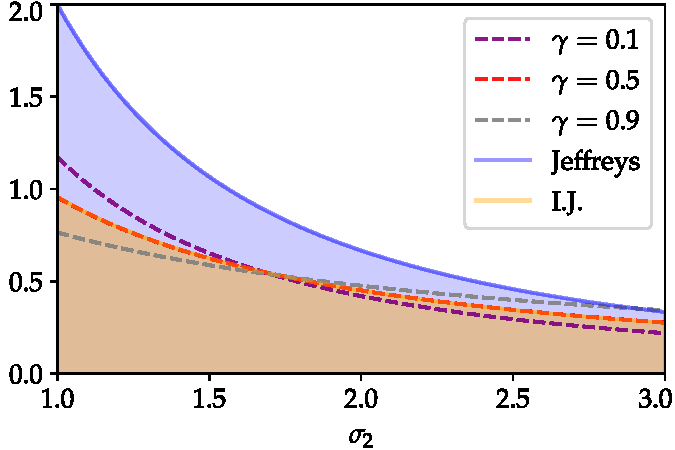
\includegraphics[width=5.7cm]{figures/constrained-priors/priors_.pdf}\hspace*{1cm}%
    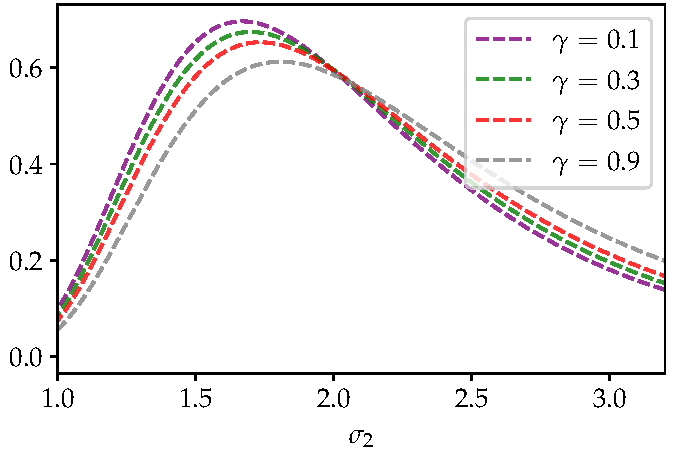
\includegraphics[width=5.7cm]{figures/constrained-priors/post5.pdf}\\
    \makebox[13cm][c]{%
    {~\hspace{\stretch{1}}(a)\hspace{\stretch{2}}(b)\hspace{\stretch{1}}~}}\\[5pt]
    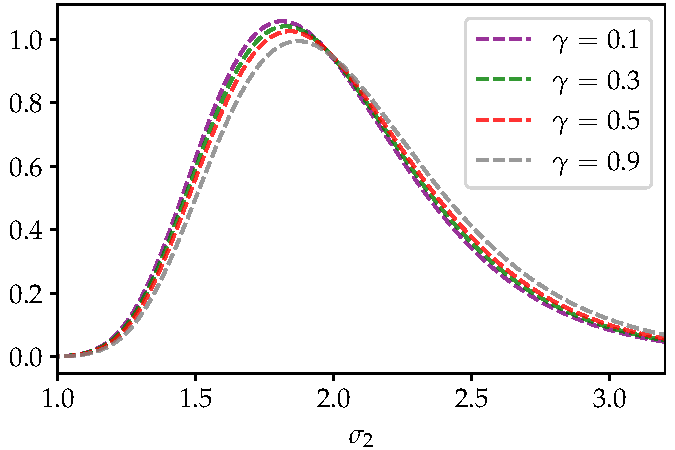
\includegraphics[width=5.7cm]{figures/constrained-priors/post15.pdf}\hspace*{1cm}%
    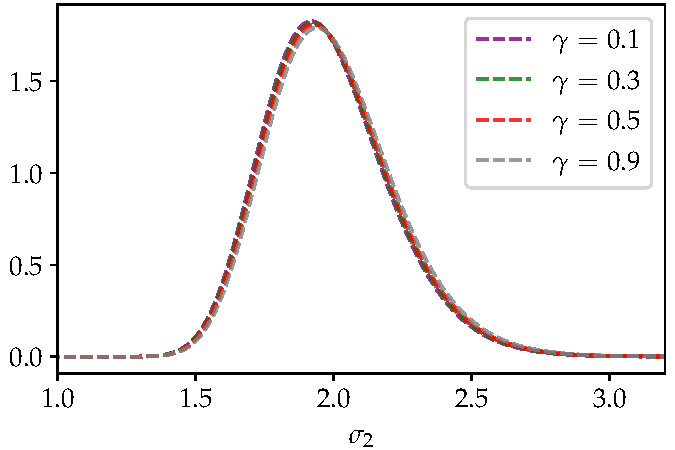
\includegraphics[width=5.7cm]{figures/constrained-priors/post50.pdf}\\
    \makebox[13cm][c]{%
    {~\hspace{\stretch{1}}(c)\hspace{\stretch{2}}(d)\hspace{\stretch{1}}~}}%
    \caption{On (a), different prior densities $\pi_\gamma$ (in dashed line) w.r.t. $\sigma_2$ along with a Jeffreys prior density (that delimits the blue area) and the \emph{Independent Jeffreys} of \cite{rubio_inference_2014} (that delimits the orange area). On each of (b), (c) and (d), posterior densities for different values of $\gamma$ are plotted. %One observed sample served the calculation of all the posteriors on one figure. 
    One observed sample was used to calculate all the posteriors in a figure.
    The observed sample has a size of $k=5$ in (b), $k=15$ in (c), and $k=50$ in (d).\label{fig:priorpost}}
\end{figure}








\section{Detailed proofs}\label{sec:BA:proofs}


\subsection{Proof of \cref{thm:Jthetaa}}

To prove this theorem, we consider to simplify the derivations that $b=0$ with $\Theta=(0,1]$. We will show later how to extend the result to the other cases. As the Jeffreys prior can be defined up to a positive multiplicative constant with no incidence on the definition of a $D_\delta$-reference prior, 
we will simplify its decay rate assuming $J(\theta)\equi{\theta\rightarrow 0}\theta^a$.

Let us define the increasing sequence of compact subsets $\Theta$: $\Theta_i=[\theta_i,1]$, $i\geq0$, with $\theta_i\conv{i\rightarrow\infty}0$. We denote by $\psi_i$ and $\tilde\psi_i$ the functions defined as follow:
    \begin{equation}
        \psi_i(u) = -\frac{\int_{\Theta_i}J(\theta)^{-\delta}\theta^{u(1+\delta)}d\theta }{\left(\int_{\Theta_i}\theta^ud\theta \right)^{1+\delta}},\qquad \tilde\psi_i(u) = -\frac{\int_{\Theta_i}\theta^{-a\delta }\theta^{u(1+\delta)}d\theta }{\left(\int_{\Theta_i}\theta^ud\theta \right)^{1+\delta}}.
    \end{equation}
The quantity $\psi_i(u)$ corresponds ---up to a positive constant--- to the parametrization w.r.t. $u\in\RR$ of $l(\pi_i)$; where $\pi(\theta)\propto\theta^u$, $\pi_i$ is re-normalized restriction of $\pi$ to $\Theta_i$  and where $l$ is the function defined in \cref{thm:BA:l(pi)} that we seek to maximize.
Therefore, if we call $u_i\in\argmax_{u\in\RR}\psi_i(u)$ for any $i$, and if the associated sequence of priors $(M(\pi_i))_i$ converge Q-vaguely to a prior $\varPi^\ast$ over $\Theta$, that would prove that $\varPi^\ast$ is a quasi $D_\delta$-reference prior.

\paragraph{The case $\mathbf{a<-1}$}
    Firstly, we assume that $a<-1$. Denote $U=(-\infty, u_m:=\frac{\delta a-1}{1+\delta})$, we want to derive an asymptotic equivalent when $i\to\infty$ of $\psi_i(u)$, uniformly w.r.t. $u\in U$.
    More precisely, we are about to show that for any $\eps>0$ there exists a $i_1$ such that for any $u\in U$ and $i>i_i$, $|\psi_i(u)-\tilde\psi_i(u)|<\eps|\tilde\psi_i(u)|$. %\theta_i^{-\delta(a+1)}$.
    

    Let $\eps>0$, using that $J(\theta)^{-\delta}\equi{\theta\rightarrow0}\theta^{-\delta a}$, there exists $i_0$ such that for any $\theta<\theta_{i_0}$, $|J(\theta)^{-\delta}-\theta^{-\delta a}|<\eps\theta^{-\delta a}$. %for a $\tilde\eps$ that we determine later.
    Now, we consider an $i_1$ such that: % for any $u\in U$:
        \begin{equation}
            \frac{\int_{\Theta_{i_0}}J(\theta)^{-\delta}d\theta }{\int_{\theta_{i_1}/\theta_{i_0}}^1J(\theta_{i_0}\theta)^{-\delta}\theta^{u_m(1+\delta)} d\theta}<\theta_{i_0}\eps/2\quad \text{and}\quad
            \frac{\int_{\Theta_{i_0}}\theta^{-\delta a}d\theta }{\int_{\theta_{i_1}/\theta_{i_0}}^1(\theta_{i_0}\theta)^{-\delta a}\theta^{u_m(1+\delta)} d\theta}<\theta_{i_0}\eps/2.
        %
            % \frac{\int_{\Theta_{i_0}} J(\theta)^{-\delta}\theta^{u(1+\delta)}  d\theta}{\int_{\Theta_{i_1}\setminus\Theta_{i_0} } J(\theta)^{-\delta }\theta^{u(1+\delta)}d\theta }
            % = 
            % \frac{\theta_{i_0}^{-1}\int_{\theta_{i_0}}^1 J(\theta)^{-\delta}(\frac{\theta}{\theta_{i_0}})^{u(1+\delta)}  d\theta}{\int_{\theta_{i_1}/\theta_{i_0}}^1 J(\theta_{i_0}\tilde\theta)^{-\delta }\tilde\theta^{u(1+\delta)} d\tilde\theta }
            % %
            % < \frac{\theta_{i_0}^{-1}\int_{\Theta_{i_0} }J(\theta)^{-\delta} d\theta}{\int_{\theta_{i_1}/\theta_{i_0} }^1 J(\theta_{i_0}\theta)^{-\delta }\theta^{u^m(1+\delta)}d\theta}
        \end{equation}
    Thus, for any $i>i_1$  and any $u\in U$:
        \begin{equation}
            \frac{\int_{\Theta_{i_0}} J(\theta)^{-\delta}\theta^{u(1+\delta)}  d\theta}{\int_{\Theta_{i}\setminus\Theta_{i_0} } J(\theta)^{-\delta }\theta^{u(1+\delta)}d\theta }
            = 
            \frac{\theta_{i_0}^{-1}\int_{\theta_{i_0}}^1 J(\theta)^{-\delta}(\frac{\theta}{\theta_{i_0}})^{u(1+\delta)}  d\theta}{\int_{\theta_{i}/\theta_{i_0}}^1 J(\theta_{i_0}\theta)^{-\delta }\theta^{u(1+\delta)} d\theta } %\\
            %
            < \frac{\theta_{i_0}^{-1}\int_{\Theta_{i_0} }J(\theta)^{-\delta} d\theta}{\int_{\theta_{i_1}/\theta_{i_0} }^1 J(\theta_{i_0}\theta)^{-\delta }\theta^{u_m(1+\delta)}d\theta} < \eps/2
        \end{equation}
    and
        \begin{equation}
            \frac{\int_{\Theta_{i_0}} \theta^{-\delta}\theta^{u(1+\delta)}  d\theta}{\int_{\Theta_{i}\setminus\Theta_{i_0} } \theta^{-\delta }\theta^{u(1+\delta)}d\theta }
            = 
            \frac{\theta_{i_0}^{-1}\int_{\theta_{i_0}}^1 \theta^{-\delta}(\frac{\theta}{\theta_{i_0}})^{u(1+\delta)}  d\theta}{\int_{\theta_{i}/\theta_{i_0}}^1 (\theta_{i_0}\theta)^{-\delta }\theta^{u(1+\delta)} d\theta } %\\
            %
            < \frac{\theta_{i_0}^{-1}\int_{\Theta_{i_0} }\theta^{-\delta} d\theta}{\int_{\theta_{i_1}/\theta_{i_0} }^1 (\theta_{i_0}\theta)^{-\delta }\theta^{u_m(1+\delta)}d\theta} < \eps/2,
        \end{equation}
    so that $|\psi_i(u)-\tilde\psi_i(u)|<\tilde\eps|\tilde\psi_i(u)|$ as expected. %Finally, deriving $\tilde\psi_i(u)$ gives
        %\begin{equation}
         %   |\psi_i(u)-\tilde\psi_i(u)|<\tilde\eps  |u+1|^\delta K\theta_i^{-\delta(a+1)}\frac{1-\theta_i^{-(\delta(u-a)+u+1)}}{(1-\theta_i^{-u-1})^{1+\delta}} <\tilde\eps |u+1|^\delta K'\theta_i^{-\delta(a+1)}
        %\end{equation}        
    %for some constants $K,\,K'>0$, using that $\theta_i^{-u-1}\leq\theta_i^{-u_m-1}<1$ and that$\theta_i^{-(\delta(u-a)+u+1)}\leq\theta_i^{-(\delta(u_m-a)+u_m+1)}\leq1$. Hence the expected result when $\tilde\eps=\eps/K$.

    Now we want to use this asymptotic equivalence to bound the difference $|a-u_i|$, where $u_i$ is defined as a maximal argument of $\psi_i$. The next step is thus to show that such $(u_i)_i$ exists.
    
    There exist $\tilde K$, $\tilde K'$ such that $\tilde K\theta^{-\delta}\leq J(\theta)^{-\delta}\leq \tilde K'\theta^{-\delta}$. 
    Let $i\geq0$, we can write
        \begin{equation}\label{eq:gendarmeJeffreys}
            \tilde K |\tilde\psi_i(u)| \leq|\psi_i(u)| \leq \tilde K'|\tilde\psi_i(u)|
        \end{equation}
    with 
        \begin{equation}
            |\tilde\psi_i(u)| = \theta_i^{-\delta(a+1)}\frac{|u+1|^{1+\delta}}{|\delta(u-a)+u+1|}\frac{1-\theta_i^{-\delta(u-a)-u-1}}{(1-\theta_i^{-u-1})^{1+\delta}}  \conv{u\rightarrow-\infty}+\infty.
        \end{equation}
    That makes $|\psi_i|$ being a coercive and continuous function on $U$, so that it admits minimal arguments in $U$. We denote by $u_i$ one of them: 
        \begin{equation}
            u_i \in \argmax_{u\in U} \psi_i(u).
        \end{equation}

    We recall that, by concavity of $x\mapsto -x^{-\delta}$, we find that $a$ is the only maximal argument of $\tilde\psi_i$ for any $i$. 
    This way, for $i>i_1$, we write
        \begin{align}
            |\tilde\psi_i(u_i)-\tilde\psi_i(a)|&\leq |\psi_i(u_i)-\tilde\psi_i(u_i)| +  |\psi_i(a)-\tilde\psi_i(a)| + |\psi_i(u_i)-\psi_i(a)| \nonumber\\
            \tilde\psi_i(a) - \tilde\psi_i(u_i) &%\leq \eps(|u_i+1|^\delta+ |a+1|^\delta) \theta_i^{-\delta (a+1)} + \psi_i(u_i)-\psi_i(a),
            \leq \eps(|\tilde\psi_i(u_i)|+|\tilde\psi_i(a)|)+ \psi_i(u_i)-\psi_i(a),
        \end{align}
    which leads to 
        \begin{align}
            2(\tilde\psi_i(a)-\tilde\psi_i(u_i)) &%\leq  \eps(|u_i+1|^\delta+ |a+1|^\delta) \theta_i^{-\delta (a+1)} + \psi_i(u_i)-\tilde\psi_i(u_i)+\tilde\psi_i(a)-\psi_i(a) \nonumber\\
            \leq \eps(|\tilde\psi_i(u_i)|+|\tilde\psi_i(a)|) +  \psi_i(u_i)-\tilde\psi_i(u_i)+\tilde\psi_i(a)-\psi_i(a) \nonumber\\
            \tilde\psi_i(a) - \tilde\psi_i(u_i) &%\leq \eps (|u_i+1|^\delta+ |a+1|^\delta) \theta_i^{-\delta (a+1)}.
            \leq \eps(|\tilde\psi_i(u_i)|+|\tilde\psi_i(a)|).
        \end{align}
    %The above work allows to conclude that
    %Within the last inequality above, 
    Consequently to the convergence of
     $(\theta_i^{\delta(a+1)}\tilde\psi_i(a))_i$ toward a positive limit when $i\to\infty$, we deduce that $\theta_i^{\delta(a+1)}(\tilde\psi_i(a)-\tilde\psi_i(u_i))/|\theta_i^{\delta(a+1)}\tilde\psi_i(u_i)|$ is asymptotically null. This prevents the sequence $(\theta_i^{\delta(a+1)}\tilde\psi_i(u_i))_i$ to admit a non finite subsequential limit, meaning it has to be bounded and to converges to the same limit as $(\theta_i^{\delta(a+1)}\tilde\psi_i(a))_i$, i.e. $-|a+1|^\delta$.

     On another hand, we notice that for any $M>0$, there exist a $M'$ such that for any $u<M'$, 
        \begin{equation}
            \frac{|u+1|^{1+\delta}}{|\delta(u-a)+u+1|}>M
        \end{equation}
     and $|\theta^{\delta(a+1)}\tilde\psi_i(u)|>M$ for any $i\geq0$. Thus, as $(\theta^{\delta(a+1)}\tilde\psi_i(u_i))_i$ has been proven to be bounded, so must be $(u_i)_i$.

     To conclude on that sequence, we denote by $\rho$ a finite subsequential limit of $(u_i)_i$, if $\rho\ne u_m$ then deriving the limit of $\theta^{\delta(a+1)}\tilde\psi_i(u_i)$ leads to 
        \begin{align}
           & -\frac{|\rho+1|^{1+\delta}}{\delta(\rho-a)+\rho+1} = |a+1|^\delta \nonumber\\
           \text{i.e.}\quad & -|\rho+1|(|\rho+1|^\delta-|a+1|^\delta) = |a+1|^\delta \delta(\rho-a);
        \end{align}
    necessarily, $\rho=a$.
    It remains to prove that $\rho=u_m$ is absurd. Indeed, in this case the integrals $\int_{\Theta_i}\theta^{-\delta a+u_i(1+\delta)}d\theta$ converge either to $0$, either to $+\infty$. Therefore, that would make $(\theta_i^{\delta(a+1)}\tilde\psi_i(u_i))_i$ converging either to $-\infty$, either to $0$, which in both case is different to $-|a+1|^\delta$.


    %Eventually, $(u_i)_i$ converges to $a$.

    Let us now work beyond the subset $U$ of $\RR$. First, if $u\in(-1,+\infty)$, the integrals that compose $\psi_i(u)$ both admit finite and positive limits when $i\to\infty$. The limit of $(|\psi_i(u)|)_i$ is moreover bounded from below as a consequence of \cref{eq:gendarmeJeffreys}:
        \begin{equation}\label{eq:minorationpsiu1infty}
            |\psi_i(u)|\geq \tilde K\frac{(u+1)^{1+\delta}}{ \delta(u-a)+u+1}\frac{1-\theta_i^{\delta(u-a)+u+1}}{(1-\theta_i^{u+1})^{1+\delta}} \geq \tilde K'|\log\theta_i|^{-1-\delta}.  %{(\mu+1)^{\delta}}. %\conv{i\rightarrow\infty}\infty
        \end{equation}
    %and the same way, $\psi_i(-1)\geq\tilde K\frac{(\log\theta_i)^{-1-\delta}}{|\delta(1+a)|}$
    Thus, there exists $i_2\geq0$ such that for any $i>i_2$ $|\psi_i(a)|<\tilde K'|\log\theta_i|^{-1-\delta}$, consequently to $\psi_i(a)\equi{i\rightarrow\infty}|a+1|^{\delta}\theta_i^{-\delta(a+1)}\aseq{i\rightarrow\infty}o(|\log\theta_i|^{-\delta-1})$.
    As a result, for any $i>i_2$:
        \begin{equation}
            \sup_{u\in(-1,+\infty)}\psi_i(u)<\psi_i(a)\leq\psi_i(u_i).
        \end{equation}
    Finally, if $u\in(u_m,-1)$, analogously than in \cref{eq:minorationpsiu1infty}, we can write
        \begin{equation}
            |\psi_i(u)|\geq\tilde K(u+1)^{1+\delta}\frac{|\log\theta_i|}{(1-\theta_i^{u+1})^{1+\delta}} \geq \tilde K''\theta_i^{-(u_m+1)(1+\delta)}|\log\theta_i|^{-\delta}.
        \end{equation}
    Once again, we have $\psi_i(a)\aseq{i\rightarrow\infty}o(\theta_i^{-(u_m+1)(1+\delta)}|\log\theta_i|^{-\delta})$ and we can consider $i_3\geq 0$ such that for any $i>i_3$:
        \begin{equation}
            \sup_{u\in(u_m,-1)}\psi_i(u)<\psi_i(a)\leq\psi_i(u_i).
        \end{equation}

    All the work that precedes proves that any sequence $(v_i)_i$ defined by $v_i\in\argmax_{\RR}\psi_i$ converges to $a$.
    

\paragraph{The case $\mathbf{a=-1}$}
In this case, we easily get that $\psi_i(a)\equi{i\rightarrow\infty}-|\log\theta_i|^{-\delta}$. 
When $u<\eta<a$, 
    \begin{equation}
        |\psi_i(u)|\geq\tilde K\frac{|u+1|^{\delta}}{\delta+1} \frac{1-\theta_i^{-(\delta+1)(u+1)}}{(1-\theta_i^{-u-1})^{1+\delta}}\geq \hat K {|\eta+1|^{\delta}}(1-\theta_i^{-(\eta-1)({1+\delta})})
    \end{equation}
and when $u>\tilde\eta>a$,
    \begin{equation}
        |\psi_i(u)|\geq\tilde K\frac{|u+1|^{\delta}}{\delta+1} \frac{1-\theta_i^{(\delta+1)(u+1)}}{(1-\theta_i^{u+1})^{1+\delta}}\geq \hat K' {|\tilde\eta+1|^{\delta}}(1-\theta_i^{(\tilde\eta-1)({1+\delta})}).
    \end{equation}


Thus, for any $\eps>0$, the equations above with $\eta=a-\eps$ and $\tilde\eta=a+\eps$ let state that there exists an $i_1\geq0$ such that for any $i>i_1$:
    \begin{equation}
        \sup_{u\in(-\infty,a-\eps)}\psi_i(u)<\psi_i(a)\quad\text{and} \quad\sup_{u\in(a+\eps,\infty)}\psi_i(u)<\psi_i(a)
    \end{equation}
so that $\argmax_{\RR}\psi_i\subset(a-\eps,a+\eps)$, which let the definition of a sequence $(u_i)_i$ of maximal arguments of $\psi_i$ which converges to $a$.


\paragraph{Q-vague convergence}
The conclusion concerning the Q-vague convergence of the $M(\pi_i^\ast)$ defined from the $u_i$ constructed in the work above: $\pi_i^\ast(\theta)\propto\theta^{u_i}$ is a direct result of \cite[Proposition 2.16]{bioche_approximation_2016}. Indeed, the convergence of sequence $(u_i)_i$ toward $a$, implies that the sequence of our priors converges Q-vaguely to $\varPi^\ast$ such that $\varPi^\ast = M(\pi^\ast)$ with $\pi^\ast(\theta)\propto{\theta^a}$.



\paragraph{Extension to other set $\Theta$}
We shall now demonstrate that the proven result extends itself to the general case: $\Theta=[c,b)$ or $(b,c]$, $b\in\RR\cup\{-\infty,\infty\}$.

We first consider $\Theta=(b,c]$ with $b\in\RR$.
We denote by $\cQ$ the set of priors densities after the substitution $\vartheta = (\theta-b)/(c-b)\in T=(0,1)$:  $\cQ=\{\tilde\pi(\vartheta) = (b-c)\pi(\vartheta (b-c)+b),\,\pi\in\hat\cR\}$.
Thus, $\cQ = \{\pi(\theta)\propto\vartheta^u,\,u\in\RR\}$.
We define the increasing sequence of compact sets $(\Theta_i)_i$ by $\Theta_i = [b+t_i,c]$ with $t_i\conv{i\rightarrow}0$. Therefore, for $\pi\in\hat\cP$, calling $\pi_i$ the renormalized restriction of $\pi$ to $\Theta_i$ gives
    \begin{equation}
        l(\pi_i) = \tilde l(\tilde\pi_i) = C_\delta\int_{T_i}\tilde\pi_i(\vartheta)^{1+\delta}\tilde J(\vartheta)^{-\delta}d\vartheta
    \end{equation}
with $T_i=[t_i,1]$, $\tilde\pi_i(\vartheta) = (b-c)\pi_i(\vartheta (b-c)+b)\in\cQ$ and $\tilde J(\vartheta) = (b-c)J(\vartheta (b-c)+b)\equi{\vartheta\rightarrow0}\vartheta^a$.
Thus, the work done above states that the family of maximal arguments $\tilde\pi_i^\ast$ of $\tilde l$ over $\cQ_i$  provides a sequence of priors $(M(\tilde\pi_i^\ast))_i$ that converges Q-vaguely toward $M(\tilde\pi^\ast)$ where $\tilde\pi^\ast(\vartheta)\propto\vartheta^a$.
Thus, the associate densities $\pi^\ast_i$ maximize $l$ over $\cP_i$ and issues a sequence of priors $(M(\pi^\ast_i))_i$ that converges Q-vaguely toward $M(\pi^\ast)$ where $\pi^\ast(\theta)\propto|\theta-b|^a$.

To treat the other cases, other substitutions with analogous work permit to conclude:
(i) the substitution $\vartheta=(b-\theta)/(b-c)$
when $\Theta=(c,b)$, $b\in\RR$; (ii) the substitution $\vartheta=1/(|\theta-c|+1)$ when 
$\Theta=[c,\infty)$ or $(-\infty,c]$.








\subsection{Proof of \cref{prop:constraints}}

Let us start by the uniqueness.
%Recall the definition of an openly increasing sequence of compact sets $(\Theta_i)_{i\in\NN}$: there exist $i_0\geq0$ and a sequence $(V_i)_{i\geq i_0}$ of open subsets of $\Theta$  such that for any $i\geq i_0$
%    \begin{equation}
%        \Theta_i\subset V_i\subset \Theta_{i+1}.
%    \end{equation}
%This way, $\bigcup_iV_i=\Theta$ and the compacity of $\Theta$ imposes it to  be a finite union, so that $\Theta_i=\Theta$ for any $i\geq i_1$ for some $i_1\geq0$.\\
%
%
%If $(\Theta_i)_{i\in \NN}$ is an increasing sequence of compact subsets that covers $\Theta$, %%%($i_1<i_2\Longrightarrow\Theta_{i_1}\subset\Theta_{i_2}$, $$), 
%it is stationary, i.e. there exist an $i_0$ such that for any $i>i_0$, $\Theta_i=\Theta$.\\ %%%finite subset $\tilde I\subset I$ such that $\bigcup_{i\in\tilde I}\Theta_i=\Theta$ (or, if $I$ is totally ordored, there exist $i_0$ such that for any $i>i_0$, $\Theta_i=\Theta$).\\
%Indeed, by contradiction assuming that for any $n$, $\bigcup_{i\leq n}\Theta_i\ne\Theta$, its complementary is non-empty and contains a non-empty closed subset $F_n\subset\left(\bigcup_{i\leq n}\Theta_i\right)^c$. Therefore, as $\Theta\subset\RR^d$ it is an Hausdorff compact set so that the two closed sets $F_n$ and $G_n=\bigcup_{i\leq n}\Theta_i$ are subsets of two disjoints open sets $U_n$ and $V_n$: $F_n\subset U_n$, $G_n\subset V_n$. This way, $\bigcup_{n\in\NN}V_n=\Theta$ and by compactness there exists $N$ such that $V_N=\Theta$ and so $F_N=\empty$ which is a contradiction.
%
%Any $D_\delta$-reference prior
A prior $\varPi^\ast\in\cP$ is a $D_\delta$-reference prior if and only if its density $\pi^\ast$ maximizes $l$ over $\cR$, where $M(\cR)=\cP$.
As the set $\cP$ is convex, $\cR$ is convex as well. Also, we notice that the function $\pi\mapsto l(\pi)$ is strictly concave, so that its maximizer is unique in the sense that two maximizer are equal $\nu$-a.e. That ensures the $D_\delta$-reference prior is unique.
%$\pi^\ast$ over a convex   such as $\tilde\cP$ must maximize $l$ as a prior on $\Theta$. The mapping $\pi\mapsto l(\pi)$ being strictly convex when $\pi$ is seen as a function in $\cR^\cC$, such maximal argument is unique.


% Regarding the expression of $\pi^\ast$,it can be seen as a direct consequence of the following lemma, which proven later on.

% \begin{lem}\label{lem:constrainstaec0}
%     Calling $U$ the set of positive and a.e. continuous function from $\Theta$ to $\RR$, and $C=\{f:\Theta\to\RR,\, \int_\Theta f=1,\,\forall j,\,\int_\Theta f_jg_j=c_j\}$, if $\pi^\ast=\argmax_{\pi\in C\cap U}l(\pi)$ exists, it verifies
%         \begin{equation}\label{eq:lemconstepiast}
%             \pi^\ast(\theta)  J(\theta)\left(\lambda_0+\sum_{j=1}^p\lambda_jg_j(\theta)\right)^{1/\delta},
%         \end{equation}
%     for some $\lambda_j\in\RR$. Reciprocally, if there exists a $\pi^\ast\in C\cap U$ that satisfies above equation for some $\lambda_j\in\RR$, then it maximizes $l$ over $C\cap U$.
% \end{lem}




% \paragraph{Proof of Lemma {lem:constrainstaec0}}
Regarding the expression of $\pi^\ast$,
let us call $E$ the space of bounded a.e. continuous functions from $\Theta$ to $\RR$ and we equip $E$ with the supremum norm over $E$: $\|f\|=\sup_\Theta|f|$. The set $\Theta$ being supposed compact, the pair $(E,\|\cdot\|)$ constitutes a Banach vector space whose restriction $U$ composed by the positive functions of $E$ is an open and convex subset.
It is possible to see $l$ as being a concave function defined on $U$.


Let us compute the differentiate of $l$ over $U$. One can write $l=\phi_2\circ\phi_1$ with
\begin{equation}
    \phi_1:\pi\in E\longmapsto \pi^{1+\delta}\in E ;\qquad \phi_2:\pi\in E\longmapsto C_\delta \int_\Theta \pi(\theta)|\cI(\theta)|^{-\delta/2}d\theta.
\end{equation}
As $\phi_2$ is a continuous linear mapping from $E$ to $\RR$, $l$ is differentiate while $\phi_1$ is, with for any $h\in E$:
    \begin{equation}
        dl(\pi) = \phi_2\circ d\phi_1(\pi).
    \end{equation}
Fix $\pi\in U$. For an $\eps>0$ there exists $\tilde\eps>0$ such that while $|x|<\|\pi\|$ and $|u|<\tilde\eps$ then $|(x+u)^{1+\delta}-x^\delta-(1+\delta)x^\delta u|<\eps|u|$. Thus for any $h\in E$ such that $\|h\|<\tilde\eps$, we have
    \begin{equation}
        \|\phi_1(\pi+h) -\phi_1(\pi)-(1+\delta)\pi^\delta h\|<\eps\|h\|.
    \end{equation}
We conclude that $\phi_1$ differentiable on $U$ with $d\phi_1(\pi)h = (1+\delta)\pi^\delta h$, for any $\pi\in U$, $h\in E$. This differentiate is additionally continuous, which makes $l$ continuously differentiable as well.

Thus, considering the additional constraint $\int_\Theta\pi(\theta)d\theta=1$, this problem can be treated applying the Lagrange multipliers theorem (see e.g. \citep{zeidler_applied_2012}) to state that there exist $\lambda_0,\dots,\lambda_p\in\RR^{p+1}$ such that
    \begin{equation}
        dl(\pi^\ast)h - \lambda\int_\Theta h(\theta)d\theta - \sum_{i=1}^p\lambda_i\int_\Theta h(\theta)g_i(\theta)d\theta = 0
    \end{equation}
for any $h\in E$. Eventually, as $dl(\pi)h=C_\delta(1+\delta)\int_\Theta\pi(\theta)^{\delta}|\cI(\theta)|^{-\delta/2}h(\theta)d\theta$, we get
    \begin{align}
        \pi^\ast(\theta) = J(\theta)\bigg(\lambda_0+\sum_{i=1}^p\lambda_ig_i(\theta)\bigg)^{1/\delta}.
    \end{align}
% with $J(\theta$

Moreover,
as $l$ is strictly concave and the constraints are linear, the second order condition for the Lagrangian states the reciprocal aspect of this result: calling $C$ the space of functions satisfying the constraints, if $\pi^\ast\in U\cap C$ satisfies the last equation above, it maximizes $l$.


%To conclude, notice that densities of non-negative priors satisfying the constraints constitute %belongs to 
%the closure of $U\cap C$, $C$ designing the set of the functions that satisfy the constraints. As $\pi^\ast$ disclosed above maximizes $l$ over $U\cap C$, with $l$ being continuous on its closure. Therefore, $\pi^\ast$ maximizes $l$ over all that latter, i.e. its associated prior is the $D_\delta$-reference prior over $\tilde\cP$.

To conclude, the elements in $\tilde\cP$ are associated to densities which belong to $E$ because $\Theta$ is compact.
They are non necessarily everywhere positive, but only supposed to be non-negative.
This set of bounded a.e. continuous and non-negative functions satisfying the constraints is actually the closure of $U\cap C$ over which $l$ is continuous.
Therefore, calling $\tilde\cP^\ast$ the set of positive priors in $\tilde\cP$, we have $\argmax_{M(\pi)\in\tilde\cP}l(\pi)=\argmax_{M(\pi)\in\tilde\cP^\ast}l(\pi)$ which is $\pi^\ast$.








\subsection{Proof of \cref{thm:lintoproper}}


Assuming that it exists, denote by $\pi^\ast$ the density of the $D_\delta$-reference prior $\varPi^\ast$ over $\overline\cP$, denote as well
    \begin{equation}
        c = \int_{\Theta}\pi^\ast(\theta)g(\theta)d\theta,\quad Z_i = \int_{\Theta_i}\pi^\ast(\theta)d\theta
    \end{equation}
for any $i\in \NN$, considering an openly increasing sequence $(\Theta_i)_{i\in\NN}$ of compact sets that cover $\Theta$ over which $1>\varPi^\ast(\Theta_i)>0$ for any $i$ such that $\Theta_i\ne\Theta$ (we show later that they exist).
In particular, $\varPi^\ast$ must be the $D_\delta$-reference prior over the set $\cP^c=\{\varPi\in\sM_{\cC}^\nu,\,\int_\Theta gd\varPi =c\}$. %\subset\cP$.

Let $i\in \NN$, if $\pi_i$ is a density on $\Theta_i$ such that 
\begin{equation}
    \int_{\Theta_i}\pi_ig + \frac{1}{Z_i}\int_{\Theta\setminus\Theta_i}\pi^\ast g = \frac{c}{Z_i},
\end{equation}
then the prior whose density $\pi$ on $\Theta$ defined by $\pi=Z_i\pi_i+\pi^\ast\indic_{\Theta\setminus\Theta_i}$ %as being proportional to $\pi_i$ on $\Theta_i$ and on $\pi^\ast$ on $\Theta\setminus\Theta_i$ 
belongs to $\cP^c$.
Therefore, denoting $\pi^\ast_i$, the renormalized restriction of $\pi^\ast$ to $\Theta_i$, $l(\pi^\ast_i)$ must be larger than $l(\pi_i)$ on $\Theta_i$ by definition of the reference prior.

Thus, $\pi^\ast_i$ is a maximal argument of $l$ under the constraints 
    \begin{equation}
        \int_{\Theta_i}\pi_i = 1,\qquad \int_{\Theta_i}\pi_i g=\frac{c}{Z_i}-\frac{1}{Z_i}\int_{\Theta\setminus\Theta_i}\pi^\ast g.
    \end{equation}
Given the result of \cref{prop:constraints}, $\pi^\ast_i$ takes the form of:
    \begin{equation}
        \pi^\ast_i = J\cdot(\lambda^{(1)}_i+\lambda^{(2)}_ig)^{1/\delta}
    \end{equation}
for some $\lambda_i^{(1)}$ and $\lambda_i^{(2)}$.

Then, denoting as well $\pi^\ast_{i+1}=J\cdot(\lambda^{(1)}_{i+1}+\lambda^{(2)}_{i+1}g)^{1/\delta}$, and reminding that $\pi^\ast_{i+1}\propto\pi^\ast_i$ on $\Theta_i$, we deduce that $\lambda^{(1)}_{i+1}=\lambda^{(1)}_{i}$ as well as $\lambda^{(2)}_{i+1}=\lambda^{(2)}_{i}$.
Eventually, $\pi^\ast\propto J\cdot (\lambda_1+\lambda_2g)^{1/\delta}$.
Thus, in the neighborhood of $b$, $\pi^\ast(\theta)\equi{\theta\rightarrow b}K\lambda_1^{1/\delta}$ for some $K\ne0$ if $\lambda_1$ is non-null, which is discordant with the satisfaction of the constraint $\int_\Theta\pi^\ast g<\infty$ in the case where $\int_\Theta Jg=\infty$ or with the constraint $\int_\Theta\pi^\ast =1$ otherwise.


Finally, $\pi^\ast$ is proportional to $Jg^{1/\delta}$ and the value of $c$ must be fixed by
\begin{equation}
    c = \left(\int_\Theta J\cdot g^{1+1/\delta}\right)\cdot\left(\int_\Theta J\cdot g^{1/\delta}\right)^{-1}.
\end{equation}

To finish the proof, we still have to show that $\varPi^\ast$ is not null on any of the $\Theta_i$, or on any of the $\Theta\setminus\Theta_i$. First, there must exist $i_0$ such that $\varPi^\ast(\Theta_{i_0})>0$, so that $\varPi^\ast(\Theta_i)>0$ for any $i\geq i_0$ and the sequence $(\Theta_i)_{i\geq i_0}$ can be considered instead of the initial one. Second, for any $i$, if $\Theta\setminus\Theta_i$ is non-empty then it has a non-empty interior, as a consequence of the definition of openly increasing sequences of compact sets. Thus, as $\varPi^\ast$ is assumed to be positive, $\varPi^\ast(\Theta\setminus\Theta_i)$ is non-null. Hence the result.



\subsection{Proof of \cref{thm:quasipostpropre}}

  Consider an openly increasing sequence of compact sets $(\Theta_i)_{i\in\NN}$ that covers $\Theta$. Let $i\in\NN$, for $\varPi$ to be a $D_\delta$-reference prior over $\cP_i$, its normalized density $\pi_i$ %---associated to its probability density on $\Theta_i$--- 
  %to be a reference prior over $\cP_i$, it 
  must maximize the function $l$ under the constraints $\int_{\Theta_i}\pi_i=1$ and $\int_{\Theta_i}\pi_i g=c_i$. Thus, according to \cref{prop:constraints}, $\pi_i$ can be written as:
     \begin{equation}
         \pi_i(\theta)\propto J(\theta)(\lambda_i^{(1)}+\lambda_i^{(2)}g(\theta))^{1/\delta},
     \end{equation}
 for some $\lambda_i^{(1)}$ and $\lambda_i^{(2)}$.
 Considering, if required, a subsequence of $(\pi_i)_{i\in\NN}$, we can assume that $\lambda_i^{(1)}$ and $\lambda_i^{(2)}$ have constant signs.
 Also, by convexity we write:%
 \newcommand{\li}[1]{\lambda_i^{(#1)}}%
     \begin{align}\label{eq:convexityConsCpig}
         c_i^\delta  & \geq \int_{\Theta_i}J(\theta)(\li1+\li2g(\theta))g(\theta)d\theta\left(\int_{\Theta_i}Jg\right)^{\delta-1}  \\
         &\geq \li1\left(\int_{\Theta_i}Jg\right)^{\delta} + \li2\frac{\int_{\Theta_i}Jg^{2} }{\left(\int_{\Theta_i}Jg\right)^{1-\delta}},\nonumber
     \end{align}
    and
    \begin{align}\label{eq:convexityConspi1}
        1 & \geq \int_{\Theta_i}J(\theta)(\li1+\li2g(\theta))d\theta\left(\int_{\Theta_i}J\right)^{\delta-1} \\
        &\geq \li1\left(\int_{\Theta_i}J\right)^\delta + \li2 \frac{\int_{\Theta_i}Jg}{\left(\int_{\Theta_i}J\right)^{1-\delta}}  . \nonumber
    \end{align}
We want to identify the possible subsequential limits of $\li1$. 
We assume that one exists in $(0,\infty]$, we can consider if required a subsequence to assume that it is the actual the limit of $\li1$. 
This way, \cref{eq:convexityConspi1} does not allow $\li2$ to be non-negative.
Thus, $\li2$ is negative and by convexity,
 %  \begin{equation}
 %       1\geq \li1\left(\int_{\Theta_i}J\right)^\delta + \li2\frac{\left(\int_{\Theta_i} Jg^{1+1/\delta}\right)^{\delta/(1+\delta)}}{\left(\int_{\Theta_i}J\right)^{1-\delta}} \left(\int_{\Theta_i}J\right)^{1/(1+\delta)}
 %   \end{equation}
 %   or
    \begin{equation}\label{eq:convixity2l2leq0}
        c_i^\delta \geq \li1\left(\int_{\Theta_i} Jg\right)^\delta +\li2 \left(\int_{\Theta_i} Jg^{1+1/\delta}\right)^\delta .
    \end{equation}
%
  %  $$\frac{1}{1+\delta}-1+\delta = \frac{\delta^2}{1+\delta}\in(0,\delta)\qquad$$
 Given that $(c_i)_i$ is bounded, and that $\int_{\Theta_i}Jg\conv{i\rightarrow\infty}\infty$ while $\int_{\Theta_i}Jg^{1+1/\delta}$ has a finite limit, we deduce that $\li2$ diverges to $-\infty$.
 However, to ensure the expression of $\pi_i$ to be well defined, we must have $\li1+\li2g(\theta)\geq0$ for any $i$ and any $\theta$. As $g$ is non-null, it necessary comes that $(\li2/\li1)_i$ is a  bounded sequence.
Therefore, 
%\begin{equation}
%    \li2 \aseq{i\rightarrow\infty} o\left(\li1\left(\int_{\Theta_i}Jg\right)^\delta\right)    
%\end{equation}
$\li2 \aseq{i\rightarrow\infty} o\left(\li1\left(\int_{\Theta_i}Jg\right)^\delta\right) $
and the right hand side in \cref{eq:convixity2l2leq0} diverges to $\infty$, which is a contradiction with $(c_i)_i$ being bounded.

As a consequence, any subsequential limit of $(\li1)_i$ must belong to $[-\infty,0]$. Without changing the notations, we can now assume that $(\li1)_i$ has a limit, which we suppose to be strictly negative firstly, also, $(\li1)_i$ can then be assumed to be always negative.
 Thus, still to ensure that $\li1+\li2g(\theta)\geq0$ for any $i$, $\theta$, and reminding that $g(\theta)\conv{\theta\rightarrow b}0$ we deduce $\frac{\li2}{|\li1|}\conv{i\rightarrow\infty}\infty$.
 Then, 
 the sequence of functions $\left(\pi_i/\li2\right)_i$ converges pointwisely to $\pi^\ast$, defined by $\pi^\ast(\theta)\propto J(\theta)g(\theta)^{1/\delta}$ with  $|\frac{1}{\li2}\pi_i(\theta)|\leq C+g(\theta)$ for some $C$, with $g$ being bounded on all compact sets. %\footnote{If $g$ is not continuous but belongs to $\cR^\cC$, it is bounded on every compact. Then, \cite[Proposition 2.16]{Bioche2016} allows to conclude.}.
According to \cite[Proposition 2.15]{bioche_approximation_2016}, what precedes implies that the sequence of priors $(M(\pi_i))_i$ converges Q-vaguely to $M(\pi^\ast)$.

Eventually, if $(\li1)_i$ admits $0$ as a subsequential limit, 
we can assume that it is its actual limit.
Consequently,  the sequence of functions $(\pi_i/\li2)_i$ converges pointwisely to the density $\pi^\ast$ while being bounded  by $g$. Therefore, the sequence of priors $(M(\pi_i))_i$ converges Q-vaguely to $M(\pi^\ast)$.
%
In any cases, $M(\pi^\ast)$ is a quasi-reference prior over $\overline\cP'$.

 
 
 
 











\section{Conclusion}\label{sec:BA:conclusion}



Prior elicitation remains an open topic in Bayesian analysis, with no solution satisfying all criteria (objectivity, computational feasibility, property, ...) simultaneously. 
In this work, we have focused on the objectivity and exploitability of priors.
Specifically, we have provided some solutions for practitioners seeking non-subjective priors, addressing the practical challenges of traditional reference priors, particularly in terms of complexity and proper aspect. Through the example we presented, we demonstrated that simple criteria can lead to the construction of reference priors that are either straightforward to formulate or proper, depending on the case.

Moreover, our results show that one cannot completely dispense with a consideration of the asymptotic properties of Jeffreys prior. This emphasizes the importance of studying this prior for a complete construction of objective priors.
Indeed, although one of our results  offers a way to define in a simpler way the reference prior when it has improper decay rates, Jeffreys' rate still have to be elucidated. Our other result requires to derive the whole Jeffreys prior.

The approximation of the latter thus becomes a problem of a prior importance. Of course, one can thoroughly focus its explicit expression, yet it can be cumbersome to derive. In the \cref{chap:varp} we propose a numerical solution for the approximation of the Jeffreys prior.














